191. \begin{figure}[ht!]
\center{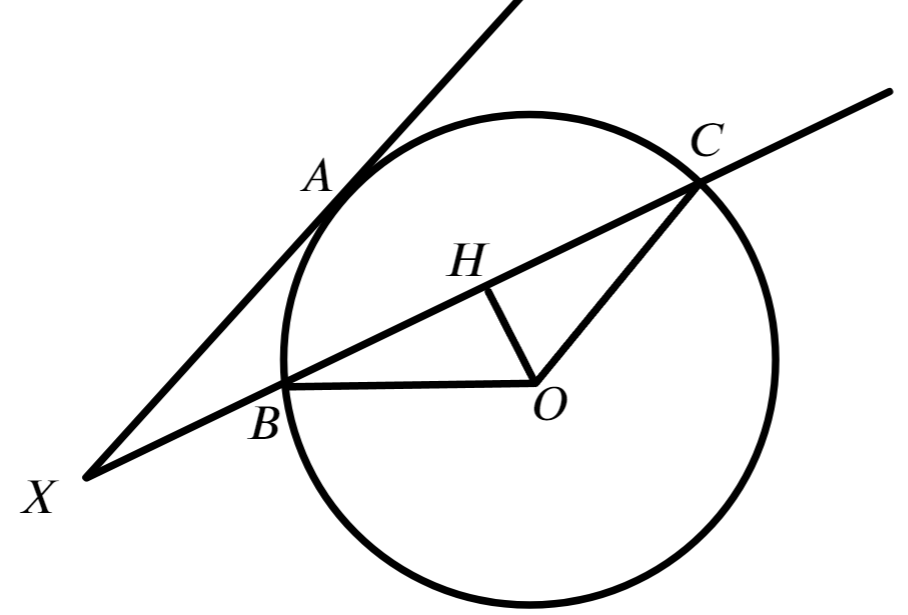
\includegraphics[scale=0.35]{g9-191.png}}
\end{figure}\\
Возможны два случая: $XB=27$ или $XC=27.$ По свойству касательной и секущей имеем равенство $XA^2=XB\cdot XC,\ 81=27XC,\ XC=3$ или $81=27XB,\ XB=3.$ В первом случае $XB>XC,$ что невозможно. Во втором случае $BC=27-3=24,$ значит $HC=24:2=12$ (треугольник $BOC$ является равнобедренным). Тогда $r=OC=\sqrt{144+25}=13.$\\
